\documentclass[12pt]{article}
\usepackage[margin=1in]{geometry}
\usepackage{graphicx}
\usepackage{amsmath}
\usepackage{tikz}
\usepackage{hyperref}
\usepackage{enumitem}

\newcommand{\biimpl}{\longleftrightarrow}
\newcommand{\impl}{\implies}

\title{CSci 8980}
\author{Yashasvi Sriram Patkuri\\Project wall-e report}

\begin{document}
\maketitle
\pagebreak

\section{Introduction}
A neural network tuned with with cross-entropy optimization method to drive a differential drive robot from start pose to a goal position.

\section{Agent design}
The state of agent is its co-ordinates and orientation $(x, y, \theta)$.
The control of agent is its linear speed and angular velocity $(v, \omega)$.
Furthermore the linear speed is clamped to be b/w $[0, v_{max}]$ and angular speed is clamped to be in b/w $[-\omega_{max}, \omega_{max}], \omega_{max} > 0$.
Here $v_{max} = 20$ and $\omega_{max} = 1$.
These were chosen by trail and error.
The $\omega_{max}$ seems to be more important than $v_{max}$ from observations.
\section{Network design}

\subsection{Input design}
For a given agent A and goal G,
Let the initial co-ordinates of A be $(x_i, y_i)$ and co-ordinates of G be $(x_g, y_g)$.
A scale S is calculated as euclidean distance b/w these points.
\[
    S = \sqrt{(x_i - x_g)^2 + (y_i - y_g)^2}
\]
Then for a given agent co-ordinates $(x_a, y_a)$, shifted-scaled co-ordinates N$(x_n, y_n)$ are calculated as follows,
\[
    N = \frac{(x_g - x_a, y_g - y_a)}{S}
\]
Observe that as the goal is fixed,
\[
    \text{agent reaches goal} \biimpl N = \bar{0}
\]
Only these co-ordinates are used for calculating rewards.
Using these co-ordinates has some advantages,
\begin{enumerate}[nolistsep]
    \item It eliminates the need of separately giving the goal co-ordinates as input.
    \item It makes the network invariant of scale of the problem.
\end{enumerate}
and some dis-advantages,
\begin{enumerate}[nolistsep]
    \item For large problem sizes, distance in terms of these co-ordinates might be low when agent is near goal hence contributing to very low rewards magnitudes.
        But this can be arbitrarily mitigated by tuning the hyper parameters of reward function.
\end{enumerate}
Along with $(x_n, y_n)$, the orientation $\theta$ of the agent is passed as input to the network. Therefore input is
\[
    (x_n, y_n, \theta)
\]

\subsubsection{Failed trials}
Per-axis scales were briefly considered. But they
\begin{enumerate}[nolistsep]
    \item Treat distances in each axis separately leading to unnatural and bad behavior.
    \item Scales become zero when agent is directly above, below, left or right of the goal, where the previous scale only becomes zero when initial position of agent and goal coincide.
\end{enumerate}

\subsection{Pipeline design}
A simple fully connected neural network with leaky ReLu activations is used.
Training process started with 2 hidden layers each with 5 nodes and leaky ReLu activations (leak = 0.1) arbitrarily which performed well during initial stages of training.

The number was increased to 3 layers during the training process when the reward functions consistently did not improve while changing all other parameters.
The final network contains 5 layers in total as illustrated in table below.
\begin{center}
\begin{tabular}{ |c|c|c| }
 \hline
 S.No. & Number of nodes & Activation \\
 \hline
 1 & 3 & identity (A(x) = x) \\
 \hline
 2 & 5 & leaky ReLu (0.1) \\
 3 & 5 & leaky ReLu (0.1) \\
 4 & 5 & leaky ReLu (0.1) \\
 \hline
 5 & 2 & identity (A(x) = x) \\
 \hline
\end{tabular}
\end{center}

\subsubsection{Other considerations}
Briefly convolution and recurrent neural networks were considered as part of pipeline.
But since the input does not have local information (like in images or text) or sequential encoded information (like in text) they were ruled out.

\subsection{Output design}
The output of network is linear speed and angular velocity at that instant.

\subsection{Parameter initialization}
While training, it was observed that initializing parameters of network uniformly randomly b/w [0, 1] gives better convergence than initializing all of them to a single value (here 0.01).

\section{Reward function design}
Each candidate network is run for multiple episodes to determine a cumulative reward and an average is taken as the reward for the candidate.

\subsection{Episode initialization}
In every episode an agent is spawned randomly in a user specified rectangle with the same candidate network.
Similarly a goal is also spawned randomly in a user specified rectangle.
The agent and goal spawning can be made deterministic by making the rectangle of zero size.
The episode runs for a user specified number of ticks

\subsection{Per episode tick rewards}
For each tick,
\begin{enumerate}[nolistsep]
    \item The input to network as described previously is created from current state.
    \item The input is given to neural network and controls are received.
    \item The controls are given to agent and scaled shifted co-ordinates N$(x_n, y_n)$ are calculated from the new state of the agent.
    \item Then the reward for the tick is calculated. It has three parts,
        \begin{enumerate}[nolistsep]
            \item Discounted angular deviation penalty.
            \item Angular velocity penalty.
            \item Shifted-scaled distance penalty.
        \end{enumerate}
    \item Tick rewards are accumulated to episode reward.
\end{enumerate}

The rewards are described below. Each of the rewards are defined so that they are bounded and scale invariant which makes it a lot easier to reason about tuning hyper parameters.

\subsubsection{Discounted angular deviation penalty}
The direction from agent to goal is defined the ideal direction for the agent.
The agent is penalized according to how far it deviates from the ideal direction.
Let the orientation of agent be $\theta$.
Let the shifted-scaled co-ordinates of agent at the new state N($(x_n, y_n$).
As N is not always a unit vector it the normalized to get $\hat{N}(\hat{x_n}, \hat{y_n})$.
Observe the vector $\hat{N}$ always points towards goal.
We use this property to define angular deviation penalty,
\[
    \Theta \equiv -\sqrt{(\hat{x_n} - cos(\theta)^2 + (\hat{y_n} - sin(\theta)^2)}
\]
It has the following advantages,
\begin{enumerate}[nolistsep]
    \item It is bounded. viz. $0 \le \Theta \le 2$.
    \item It is simpler than using atan2 variants and just as good.
    \item It is problem scale invariant.
\end{enumerate}

But if the reward from this is accumulated as-is the agent tends to just orient towards goal and stop especially near the goal where the distance rewards contributes much less. So a tick discounted variant of angular deviation penalty is used which is defined as follows,
\[
    \Theta \equiv -\frac{\sqrt{(\hat{x_n} - cos(\theta)^2 + (\hat{y_n} - sin(\theta)^2)}}{1 + \text{tick}}
\]
This mitigates the problem while retaining the advantages.

\subsubsection{Angular velocity penalty}
After training agent tends to rotationally jitter a lot as there is no restriction on angular acceleration.
To avoid this a penalty is assigned for agent corresponding to its angular velocity magnitude.
Therefore angular velocity penalty,
\[
    \Omega \equiv -|\omega|
\]
Notice that this reward is also bounded and problem scale invariant.

\subsubsection{Shifted-scaled distance penalty}
To make the agent go towards goal a penalty is assigned to agent according to distance from the goal.
But if raw co-ordinates are used there is no bound on the penalized which can drown out or be drowned by other penalties.
Therefore scale-shifted co-ordinates are used to calculate distance penalty.
Observe the magnitude of scale-shifted co-ordinates is linearly proportional to distance b/w goal and agent.
So we define, scale-shifted distance penalty as,
\[
    \Delta \equiv -k * \sqrt{x_n^2 + y_n^2}
\]
where $k$ is a positive tunable constant.
Higher values of $k$ give more importance to reducing distance.
Notice that this reward is also bounded and problem scale invariant.

\subsection{End of episode rewards}
After an episode ends, three more rewards are added to agent defined as follows,
\[
    \Phi_1 \equiv  q * e^{-\sqrt{x_n^2 + y_n^2}}
\]
where $q$ is a positive tunable constant.
\[
    \Phi_2 \equiv  r * e^{-|v|} * e^{-\sqrt{x_n^2 + y_n^2}}
\]
\[
    \Phi_3 \equiv  s * e^{-|w|} * e^{-\sqrt{x_n^2 + y_n^2}}
\]
where $r$ and $s$ are positive tunable constants.
These rewards are high when the agent reaches goal and stays there at the end of the episode.
Due to these, the agent tends to stop at or near the goal in most models without any manual intervention.

These rewards performed well enough for different settings of agent and goal.
Some models even performed well for settings they were not trained for.
This finalized the reward function for the time being.

\section{Training}
Below are a few lessons learnt during the process.
\begin{enumerate}[nolistsep]
    \item Have enough ticks in each episode for agent to reach the goal.
    \item Have enough number of generations, a good generation might come after a lot of flat generations.
    \item The hyper parameters should be such that they give a good model (and not get stuck at bad minima) frequently.
\end{enumerate}


\section{Parallelization}
During optimization, a batch of networks is generated from a seed network and rewards are calculated for each of them which will later be used.
By profiling it was found that this step takes the most amount of time.
And as reward for each candidate in batch is independent of others, it can be calculated in a parallel thread.
This simple parallelization allows for a significant speed up.
The following figure shows the speedup of parallelized implementation on a 4-core and 8-core machine compared to non-parallelized implementation for a (500 generation, 100 batch, 6 episodes per candidate, 500 ticks per episode) optimization.

\begin{figure}[h!]
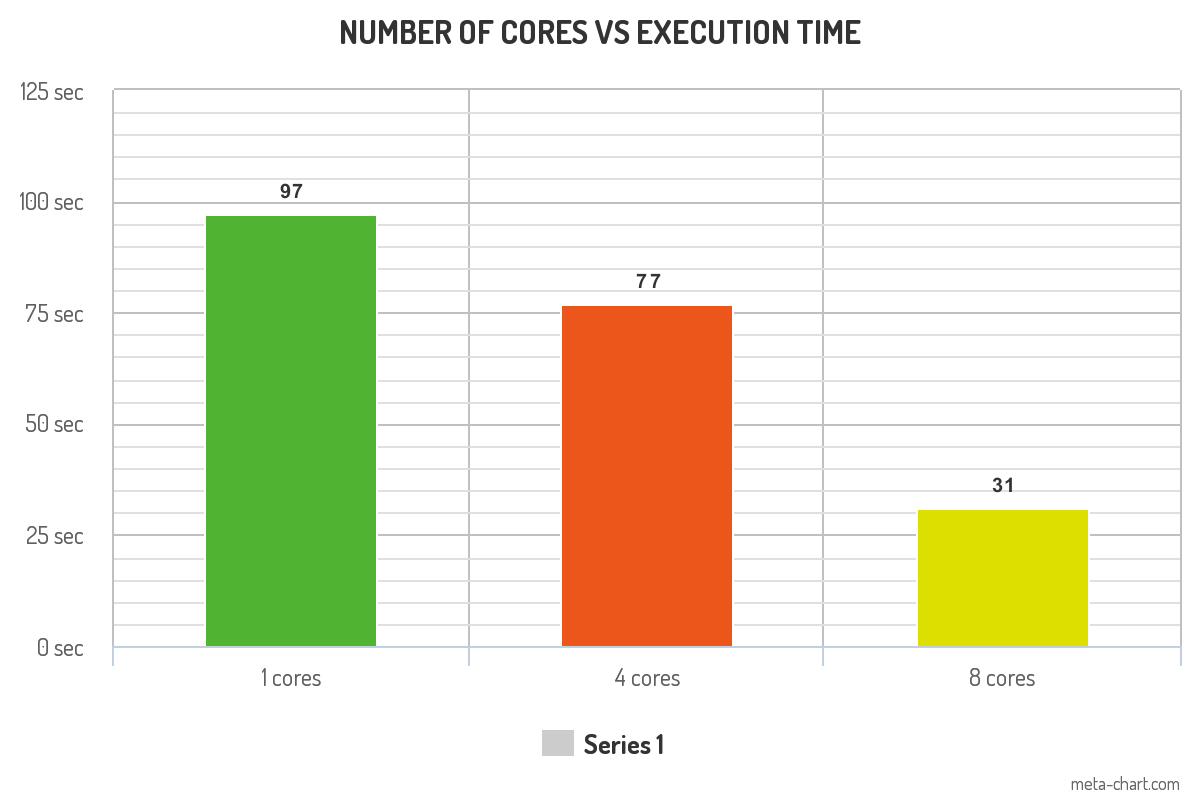
\includegraphics[width=15cm]{parallelize.png}
\centering
\end{figure}

There is 2.48x and 3.13x speedup on 4-core and 8-core machines respectively compared to serial implementation.

\subsection{Compiler optimization}
Although parallelization has its role, simple compiler optimization can do wonders.
Before compiler optimization my rust implementation was slower than python variant, whereas after full compiler optimization it is much faster.

\end{document}
